\chapter{Аналитический раздел}

В данном разделе приводится анализ предметной области и существующих решений, формулируются требования к БД и ПО, формализуется и описывается информация, подлежащая хранению в проектируемой БД, и пользователи. На основе приведенного анализа строятся диаграмма вариантов использования и ER-диаграмма сущностей в нотации Чена.

\section{Анализ предметной области и существующих решений}

Предметная область включает в себя производственные процессы на тракторном заводе: контроль производства, техническое обслуживание, учет запасов запчастей и другие аспекты, связанные с производством сельскохозяйственной техники.

Система мониторинга позволяет следить за работой оборудования. Оператору не придётся каждый раз идти к станку, чтобы узнать, как он работает и всё ли с ним в порядке. Это повышает эффективность работы персонала, особенно при большом парке оборудования. 

Собранная информация, кроме того, позволяет планировать и вовремя проводить техобслуживание и ремонты, что позволяет снизить простои и издержки.

% тут лучше перефразировать а то слово в слово скопипастил с инета 
Еще одна из задач систем мониторинга -- идентификация работника и действий, производимых на станке: собирается информация о том, какая партия изделий была произведена, на каком станке, за какое время и кто был оператором оборудования. Для своевременного обслуживания важно собирать данные об износе оборудования.

Среди уже существующих проектов, решающих поставленную задачу, для сравнения были выделены три аналога: Winnum, DPA и AF Monitor. Сравнение проводилось по ряду критериев, а именно наличие возможности просмотра общей информации о производстве, контроль и регистрация времени и причин простоев и регистрация заявок на техобслуживание. Результаты сравнения приведены в таблице \ref{tab:functionality_comparison}.



\begin{table}[H]
  \centering
  \caption{Сравнение функциональности систем AF, DPA и Winnum}
  \label{tab:functionality_comparison}
  \small
  \begin{tabular}{|c|c|c|c|}
    \hline
    & \textbf{AF} & \textbf{DPA} & \textbf{Winnum} \\
    \hline
    Просмотр информации о производстве & + & + & + \\
    \hline
    Регистрация времени и причин простоев & + & + & + \\
    \hline
    Регистрация заявок на техобслуживание & - & - & - \\
    \hline
  \end{tabular}
\end{table}

Как видно в таблице \ref{tab:functionality_comparison}, рассмотренные решения не предоставляют функционал для регистрации заявок на проведение технического обслуживания производственных линий. Таким образом, данная работа отличается от существующих решений тем, что она
удовлетворяет всем установленным критериям.


\section{Формализация и описание информации, подлежащей хранению в проектируемой базе
данных}

% перефразировать для антиплагиата 
Основываясь на анализе предметной области, можно выделить следующие сущности:

\begin{itemize}[label=--]
    \item трактор;
    \item производственная линия;
    \item сотрудник;
    \item запчасть;
    \item заказ запчастей;
    \item заявка на обслуживание;
    \item отчет об обслуживании.
\end{itemize}

В таблице \ref{tab:er} приведены сведения о рассматриваемых сущностях.

На рисунке \ref{img:er} приведена ER-диаграмма сущностей в нотации Чена.


\begin{table}[H]
    \centering
    \begin{tabular}{|c|c|} \hline 
        \textbf{Сущность} &  \textbf{Сведения}\\ \hline 
        трактор \multirow{3}{*}{} 
        & модель, год выпуска, тип двигателя,\\
        & модель двигателя, мощность двигателя,\\
        & экологическая норма выброса, емкость \\
        & топливного бака, колесная формула, \\
        & размер шин задних колес, размер шин \\
        & передних колес, длина, ширина, высота\\
        & по кабине \\ \hline

        производственная линия
        \multirow{3}{*}{} 
        & название, длина, ширина, высота, \\
        & состояние, производство (тр/мес), \\
        & простой, частота техосмотров, дата \\
        & последнего техосмотра, дата \\
        & следующего техосмотра, процент брака \\ \hline

        сотрудник
        \multirow{3}{*}{} 
        & имя, фамилия, отчество, e-mail,\\
        & пароль, дата рождения, отдел, роль, \\
        & пол \\ \hline

        запчасть
        \multirow{3}{*}{} 
        & название, длина, ширина, высота, \\
        & страна производитель, количество\\
        & на складе, цена \\ \hline

        заказ запчастей
        \multirow{3}{*}{} 
        & статус, стоимость, дата заказа, \\
        & сотрудник, заявка \\ \hline

        заявка на обслуживание
        \multirow{3}{*}{} 
        & статус, тип, дата, описание, \\
        & производственная линия, сотрудник \\ \hline

        отчет об обслуживании
        \multirow{3}{*}{} 
        & производственная линия, заявка,\\
        & сотрудник, дата начала обслуживания,\\
        & дата завершения обслуживания, цена \\
        & ремонта, описание проделанных работ \\ \hline
    \end{tabular}
    \caption{Описание сущностей}
    \label{tab:er}
\end{table}

\begin{figure}[H]
    \centering
    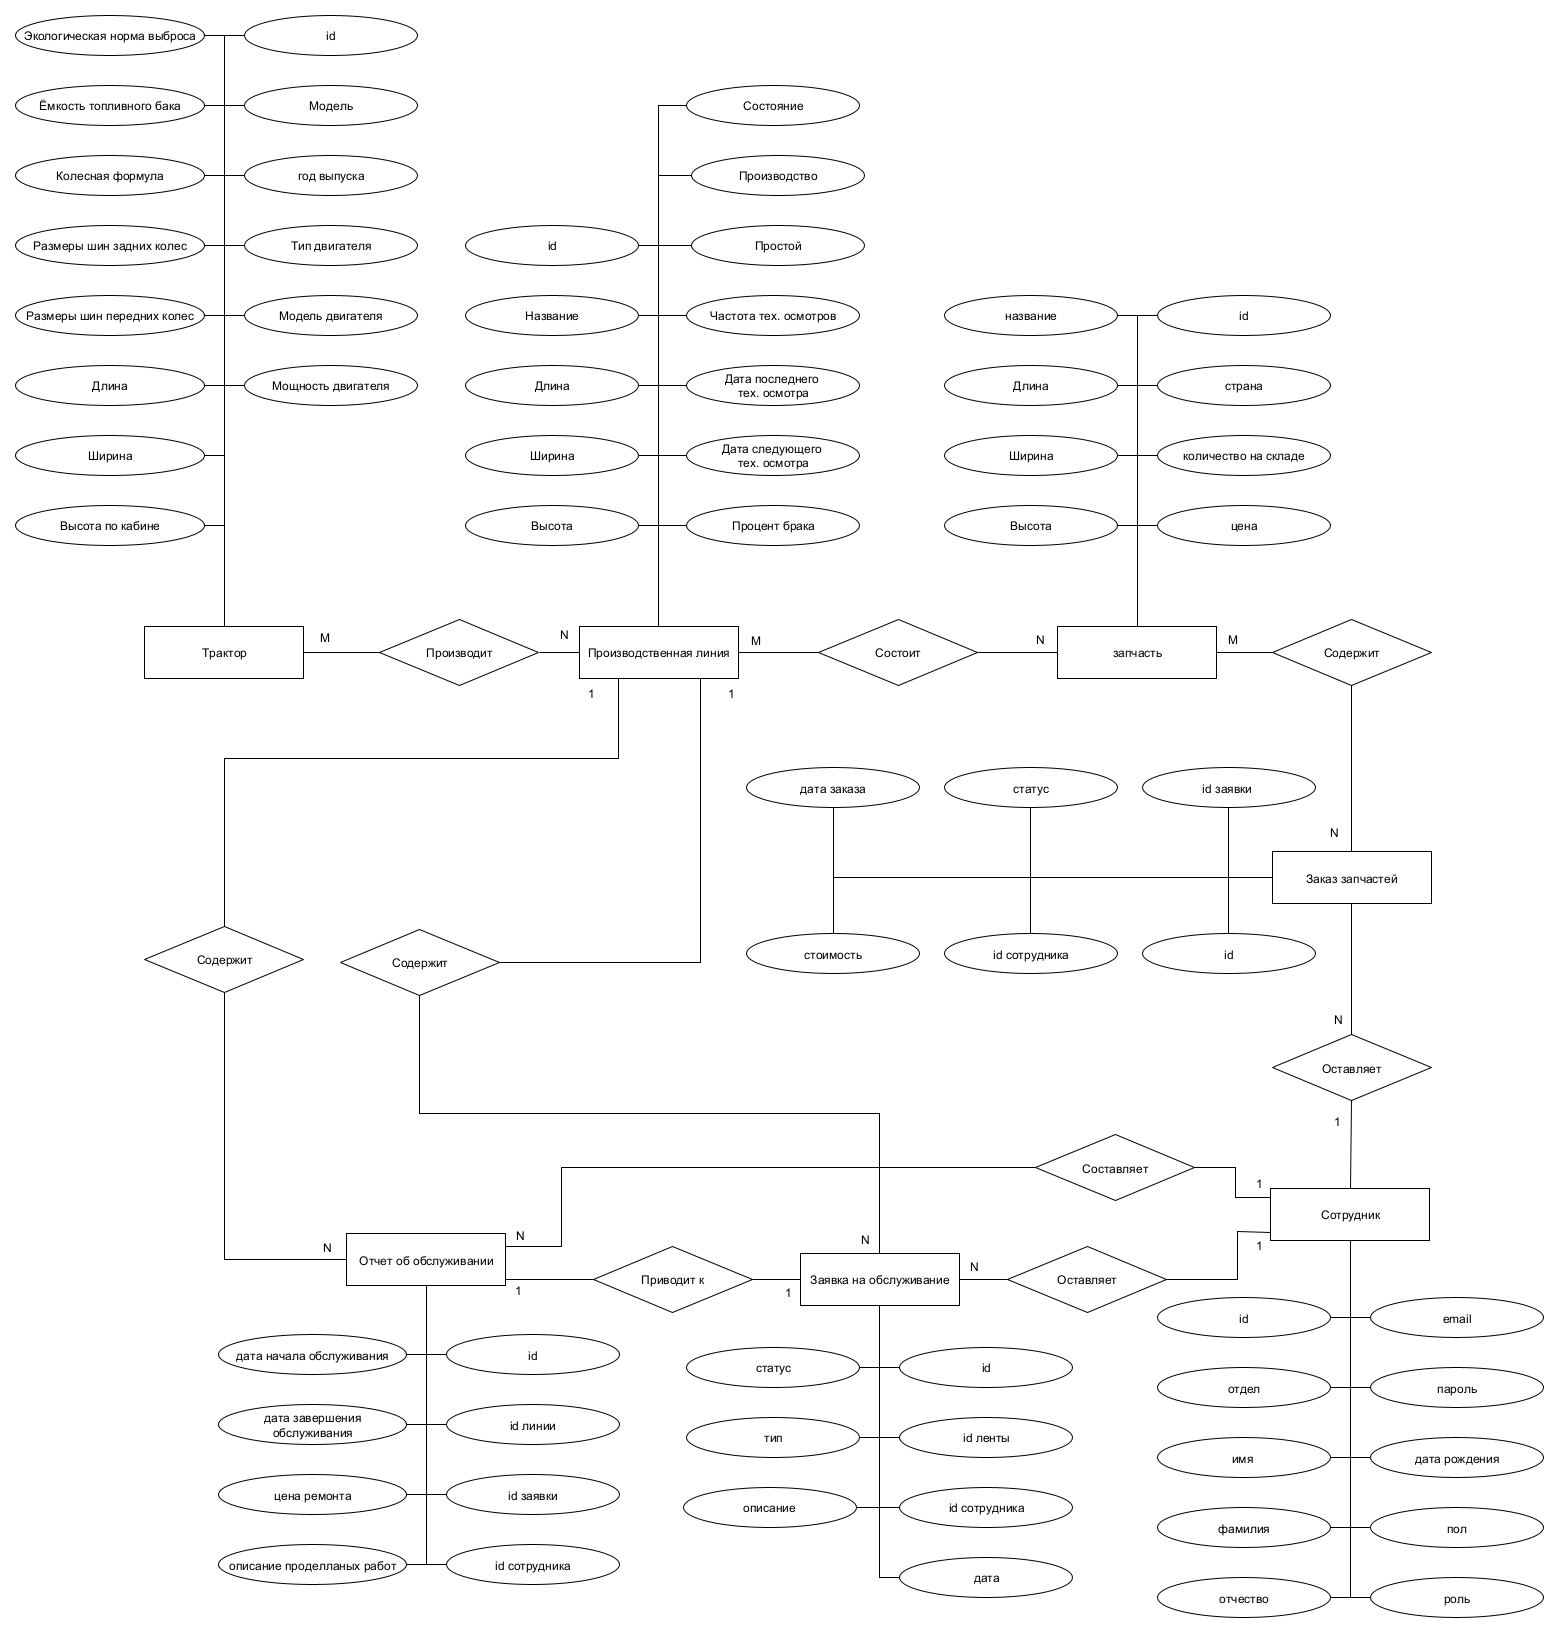
\includegraphics[width=1\textwidth]{inc/img/erchena}
    \caption{ER-диаграмма сущностей в нотации Чена}
    \label{img:er}
\end{figure}

\section{Формализация и описание пользователей}

В проектируемом приложении к базе данных выделим четыре типа пользователей:

\begin{itemize}[label=--]
    \item оператор производства -- это сотрудник предприятия, контролирующий функционирование производственных линий. Он может просматривать информацию о тракторах и производственных линиях, создавать заявки на обслуживание и изучать отчеты об обслуживании;
    \item специалист по обслуживанию -- это сотрудник, отвечающий за техническое обслуживание производственных линий, их техосмотры и ремонт. Он может просматривать информацию о производственных линиях и запчастях на складе, просматривать журнал обслуживания производственных линий, заказывать запчасти и регистрировать выполненное обслуживание заполняя отчет;
    \item администратор -- это сотрудник, отвечающий за выдачу прав доступа к системе другим сотрудникам, он может просматривать информацию о зарегистрированных пользователях и менять уровень доступа отдельных сотрудников;
    \item неавторизованный пользователь -- это пользователь не вошедший в систему, он может войти, введя свой логин и пароль, или зарегистрироваться в системе.
\end{itemize}

На рисунке \ref{img:use-case} представлена диаграмма вариантов использования.

\begin{figure}[H]
    \centering
    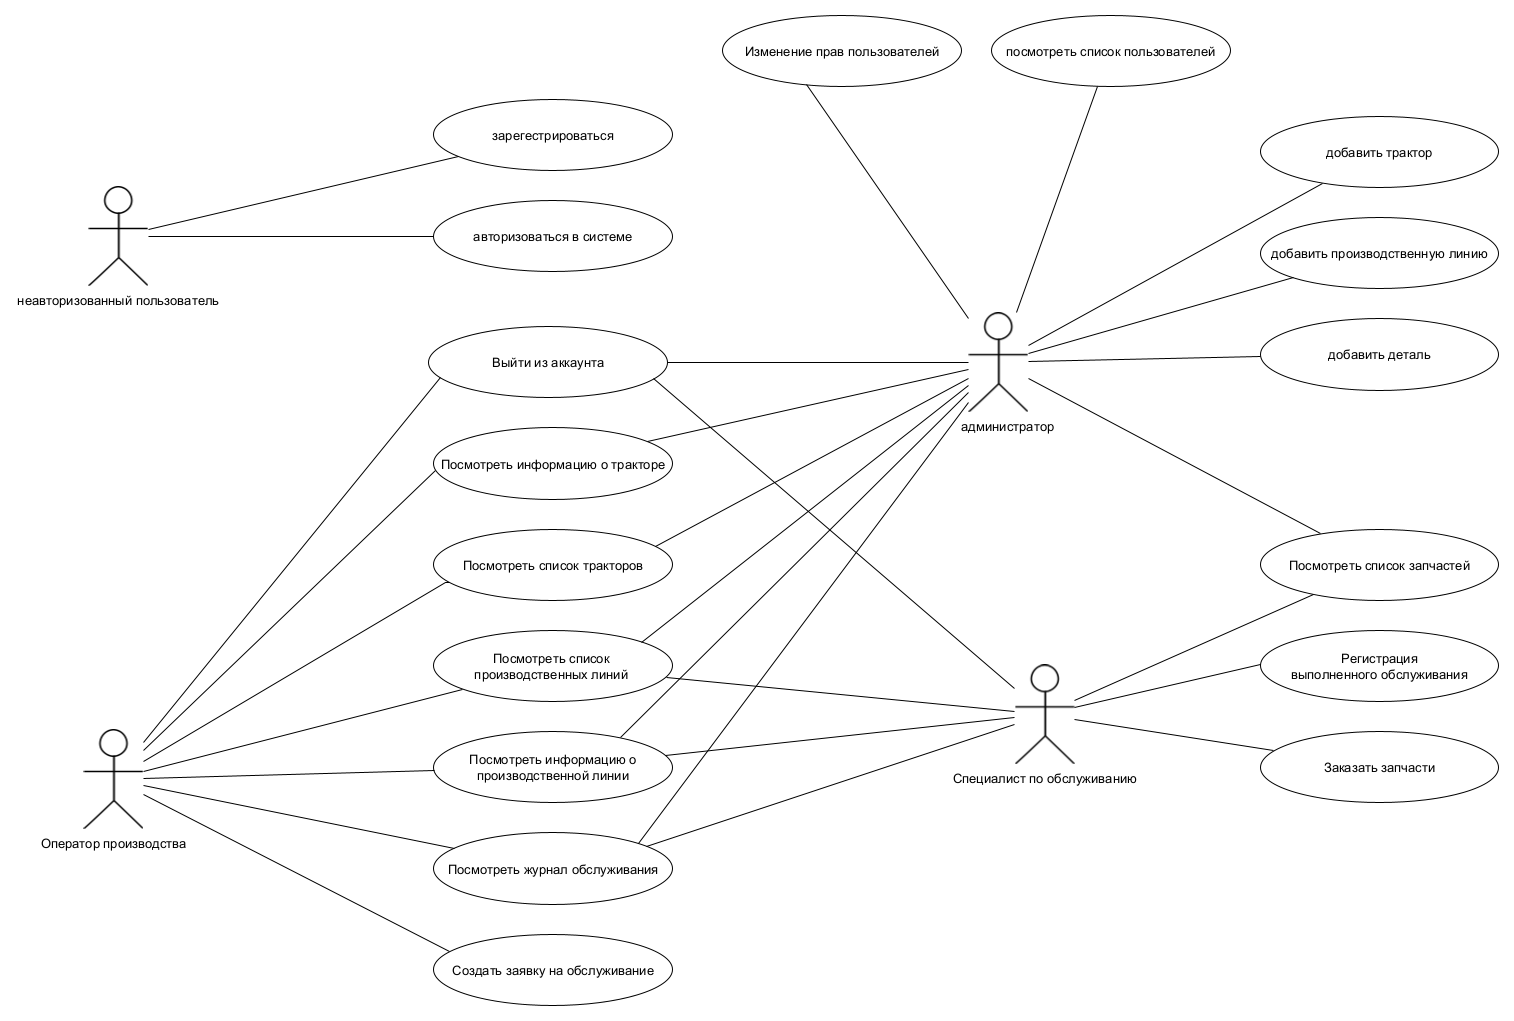
\includegraphics[width=1\textwidth]{inc/img/use-case.png}
    \caption{Диаграмма вариантов использования}
    \label{img:use-case}
\end{figure}

\section{Анализ моделей баз данных}

База данных -- это некоторый набор перманентных (постоянно хранимых) данных, используемых прикладными программными системами какого-либо предприятия\cite{дейт2001введение}. 

Система управления базой данных (СУБД) -- совокупность программ, с помощью которых осуществляются управление структурой базы данных и контроль доступа к данным, хранящимся в ней\cite{роб2004системы}.

Модель данных -- это абстрактное, самодостаточное, логическое определение объектов, операторов и прочих элементов, в совокупности составляющих абстрактную машину доступа к данным, с которой взаимодействует пользователь\cite{дейт2001введение}.

По модели данных СУБД делятся на дореляционные, реляционные и постреляционные.

\subsection{Дореляционные модели}

Основные типы дореляционных моделей\cite{дейт2001введение}:

\begin{itemize}[label=--]
    \item инвертированные списки;
    \item иерархические;
    \item сетевые.
\end{itemize}

\subsubsection{Инвертированные списки}
Модель управления данными на основе инвертированных списков является широко распространённой в современных реляционных системах управления базами данных (СУБД)\cite{кузнецов1998основы}. Однако, в таких системах пользователи не имеют прямого доступа к инвертированным спискам, которые являются внутренней структурой для управления доступом к данным.

База данных, построенная на основе инвертированных списков, схожа с реляционной БД, но отличается тем, что пользователи могут видеть как сами таблицы, так и пути доступа к ним.

Строки таблиц упорядочены в некоторой физической последовательности.
Физический порядок строк может быть определен как для каждой отдельной таблицы, так и для всей базы данных в целом.
Для каждой таблицы можно определить произвольное количество ключей поиска, для которых автоматически создаются индексы. Эти индексы поддерживаются системой и могут быть видны пользователям.

В этой модели поддерживаются два класса операторов: операторы, устанавливающие адрес записи и операторы, находящие запись относительно предыдущей записи по некоторому пути доступа.


\subsubsection{Иерархические модели}
Иерархическая модель БД состоит из объектов с указателями от родительских объектов к потомкам, соединяя вместе 
связанную информацию. Иерархические БД могут быть представлены как дерево.

На самом высшем (первом) уровне иерархии находится только одна
вершина, которая называется корнем дерева. Эта вершина имеет связи с вершинами второго уровня, вершины второго уровня имеют
связи с вершинами третьего уровня и т.д. Связи между вершинами одного уровня отсутствуют. Следовательно, данные в иерархической
структуре не равноправны – одни жестко подчинены другим. Доступ к информации возможен только по вертикальной схеме, начиная с
корня, так как каждый элемент связан только с одним элементом на верхнем уровне и с одним или несколькими на низком. Примером иерархической структуры может служить книга, как иерархическая последовательность букв, которые объединяются в слова,
слова – в предложения, предложения – в параграфы, затем в главы и т.д


\subsubsection{Сетевые модели}
Дальнейшим развитием иерархической модели является сетевая. Сетевая модель -- это структура, у которой любой элемент может быть связан с любым другим элементом\cite{интуит}.
К основным понятиям сетевой модели БД относятся: элемент (узел), связь. Узел -- это совокупность атрибутов данных, 
описывающих некоторый объект. Сетевые БД могут быть представлены в виде графа. В сетевой БД логика процедуры 
выборки данных зависит от физической организации этих данных. Поэтому эта модель не является полностью 
независимой от приложения. Другими словами, если необходимо изменить структуру данных, то нужно изменить и 
приложение.

\subsection{Реляционные модели}

Реляционная модель данных включает следующие компоненты: 
\begin{itemize}[label=--]
    \item Структурный (данные в базе данных представляют собой набор отношений);
    \item Целостностный (отношения (таблицы) отвечают определенным условиям целостности);
    \item Манипуляционный (манипулирования отношениями осуществляется средствами реляционной алгебры и/или реляционного исчисления). Кроме того, в состав реляционной модели данных включают теорию нормализации.
\end{itemize}

Реляционная модель данных является совокупностью данных и состоит из
набора двумерных таблиц. При табличной организации отсутствует иерархия
элементов. Таблицы состоят из строк -- записей и столбцов -- полей. На
пересечении строк и столбцов находятся конкретные значения. Для каждого
поля определяется множество его значений.

\subsection{Постреляционные модели}

Постреляционная модель является расширением реляционной модели\cite{БГЭУ}. Она снимает ограничение неделимости данных, допуская многозначные поля, значения которых состоят из подзначений, и набор значений воспринимается как самостоятельная таблица, встроенная в главную таблицу.

Достоинством постреляционной модели является возможность представления совокупности связанных реляционных таблиц одной постреляционной
таблицей. Это обеспечивает высокую наглядность представления информации и повышение эффективности ее обработки\cite{парфенов2016постреляционные}.

\subsection*{Вывод}

В данном разделе приводится анализ предметной области и существу-
ющих решений,  формализуется и описывается информация, подлежащая хранению в проектируемой БД, и пользователи. На основе приведенного анализа строятся диаграмма вариантов использования и ER-диаграмма сущностей в нотации Чена. 